\chapter{血液与循环系统}\label{ch:b2:blood-circulation}

1628 年，威廉·哈维算了一笔账。
他估计心脏容纳约两盎司\omterm{def:b2:blood-circulation:blood}{血液}，每分钟搏动七十次；
即使每次只射出其中一小部分，
一小时内心脏泵出的血量仍将是全身重量的数倍。
\omterm{def:b2:blood-circulation:blood}{血液}不可能按这样的速率生成和消耗，
正如盖伦在此前十四个世纪里所教导的那样；
它必定是周而复始地循环。
随后他加以证明：在手臂上扎一根绳子，绳子下方的\omterm{def:b2:blood-circulation:vessels}{静脉}会鼓起，
而上方不会；把\omterm{def:b2:blood-circulation:vessels}{静脉}里的\omterm{def:b2:blood-circulation:blood}{血液}朝手的方向挤压，
越过瓣膜时便挤不过去。\omterm{def:b2:blood-circulation:blood}{血液}经\omterm{def:b2:blood-circulation:vessels}{动脉}被泵出，经\omterm{def:b2:blood-circulation:vessels}{静脉}回流，
全部五升\omterm{def:b2:blood-circulation:blood}{血液}每分钟都要流经心脏一次。本章讨论的正是这个封闭系统：\omterm{def:b2:blood-circulation:blood}{血液}是什么，它如何被分配，
\omterm{def:b2:blood-circulation:blood}{血液}从主\omterm{def:b2:blood-circulation:vessels}{动脉}流到\omterm{def:b2:blood-circulation:vessels}{毛细血管}的流动物理学，
以及\omterm{def:b2:blood-circulation:vessels}{毛细血管}中的交换——
那才是这一切的根本目的。

\section{血液}

\begin{definition}[血液的组成]\label{def:b2:blood-circulation:blood}
\index{血液}\index{血浆}\index{血细胞比容}\index{红细胞}\index{血小板}
血液是一种悬浮态的组织：成人体内约 \qty{5}{L}，
占体重的 \qty{7}{\%}。离心分离后，血液分为
\emph{血浆}（占 \qty{55}{\%}，含水、\qty{70}{g/L} 蛋白质——
\omterm{thm:b2:blood-circulation:oncotic}{白蛋白}、球蛋白和\omterm{prop:b2:blood-circulation:clotting}{纤维蛋白}原——
以及血液所运输的盐类、糖类、脂质、
气体和激素）和血细胞（占 \qty{45}{\%}，即
\emph{血细胞比容}）：
\emph{红细胞}（每升 $5\times 10^{12}$ 个，为无核的双凹圆盘，
直径 \qty{7}{\micro m}，每个细胞内充满 2.8 亿个血红蛋白分子，
寿命 120 天，在骨髓中以每秒两百万个的速率生成）、
\emph{白细胞}（每升 $7\times 10^{9}$ 个，包括中性粒细胞、\omterm{prop:b2:blood-circulation:exchange}{淋巴}细胞、
单核细胞、嗜酸性粒细胞和嗜碱性粒细胞，是免疫的机动力量）以及
\emph{血小板}（每升 $3\times 10^{11}$ 个，是骨髓细胞的碎片，
能封堵伤口并启动凝血）。红细胞运载氧气——在完全饱和时，
每升血液可携带 \qty{200}{mL} 氧气，是水中溶解量的七十倍——
血浆则运载其余一切，包括不在细胞内的 \qty{20}{\%} 的 $\mathrm{CO_2}$、
从肌肉输向皮肤的热量，以及\cref{ch:b2:cell-signalling}中的激素，
把它们送往各自的靶点。血液同时也是一种处于\emph{\omterm{thm:b2:blood-circulation:oncotic}{胶体渗透压}}下的溶液：
其中的蛋白质不能离开\omterm{def:b2:blood-circulation:vessels}{毛细血管}，
产生约 \qty{25}{mmHg} 的渗透吸引力，
正是这一吸引力使血浆
留在血管内。
\end{definition}

\begin{omfigure}
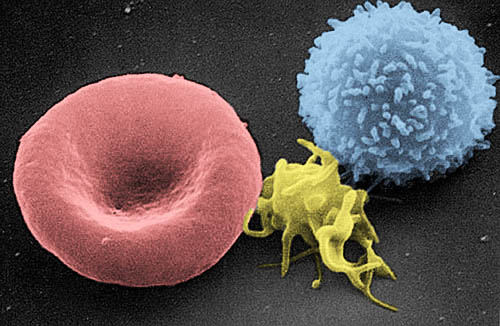
\includegraphics[width=0.5\linewidth]{images/book3/red-cells-nci.jpg}

{\small 扫描电子显微镜下的\omterm{def:b2:blood-circulation:blood}{红细胞}、\omterm{def:b2:blood-circulation:blood}{血小板}
和白细胞（\omterm{prop:b2:blood-circulation:exchange}{淋巴}细胞）：\omterm{def:b2:blood-circulation:blood}{血液}的三种细胞成分，
按相同比例绘制。}
\end{omfigure}

\begin{proposition}[止血]\label{prop:b2:blood-circulation:clotting}
\index{止血}\index{凝血级联}\index{纤维蛋白}
割伤的血管在数分钟之内被封闭，分三步完成。
血管收缩；\omterm{def:b2:blood-circulation:blood}{血小板}黏附在暴露的胶原蛋白上，
释放信号，募集并激活更多\omterm{def:b2:blood-circulation:blood}{血小板}，形成栓子；
随后，一连串\omterm{def:b2:blood-circulation:blood}{血浆}蛋白酶构成\emph{级联}，每一级激活下一级
（约十二种凝血因子，多数在肝脏中合成，其中数种需要维生素 K），
把\omterm{prop:b2:blood-circulation:clotting}{纤维蛋白}原转化为不溶的\emph{\omterm{prop:b2:blood-circulation:clotting}{纤维蛋白}}，
\omterm{prop:b2:blood-circulation:clotting}{纤维蛋白}的细丝把栓子交织成血凝块。级联具有放大作用：
受损血管壁释放的微量组织因子，最终可生成数克\omterm{prop:b2:blood-circulation:clotting}{纤维蛋白}。
这一过程还须加以控制：\omterm{def:b2:blood-circulation:blood}{血浆}中的抗凝剂（抗凝血酶、蛋白 C）
以及完好的内皮能将血凝块限制在伤口处，
而在血管愈合的过程中，另一套系统——\omterm{prop:b2:blood-circulation:clotting}{纤维蛋白}溶解——会将其溶解。
血友病是缺乏某一种因子所致；血栓则是在不需要的地方形成血凝块，
而富裕国家的首要死因，
正是冠状\omterm{def:b2:blood-circulation:vessels}{动脉}或脑\omterm{def:b2:blood-circulation:vessels}{动脉}中的血凝块。
\end{proposition}

\section{循环回路}

\begin{definition}[开放式与封闭式，单循环与双循环]\label{def:b2:blood-circulation:circuits}
\index{开放式循环}\index{封闭式循环}\index{双循环}\index{肺循环}\index{体循环}
在\emph{开放式}循环中（见于昆虫、大多数软体动物），
心脏将\omterm{def:b2:blood-circulation:blood}{血液}泵入体腔，\omterm{def:b2:blood-circulation:blood}{血液}直接浸润各器官，然后以低压回流；
血流缓慢且方向不定，昆虫则通过把空气直接导送至组织，
使气体问题与\omterm{def:b2:blood-circulation:blood}{血液}分开。在\emph{封闭式}循环中（见于环节动物、头足类和脊椎动物），
\omterm{def:b2:blood-circulation:blood}{血液}始终留在血管内，在压力作用下流经\omterm{def:b2:blood-circulation:vessels}{毛细血管}，
因而可以按器官分别进行调控。鱼类具有\emph{单循环}：
心脏 $\to$ 鳃 $\to$ 身体 $\to$ 心脏，
\omterm{def:b2:blood-circulation:blood}{血液}经鳃\omterm{def:b2:blood-circulation:vessels}{毛细血管}之后压力已经很低，
因而以低压抵达组织。
哺乳动物和鸟类具有\emph{双循环}：
右心驱动\emph{肺循环}（肺部，压力低，收缩压 \qty{25}{mmHg}），
左心在\omterm{def:b2:blood-circulation:blood}{血液}回流之后驱动\emph{体循环}
（全身，压力高，\qty{120}{mmHg}）；
两个泵串联，
输送相同的血流，静息时每分钟约 \qty{5}{L}。
两栖动物和大多数爬行动物的心脏只有一个心室，
使两股血流部分混合，这是过渡阶段。
双循环使恒温代谢成为可能：
每个器官都获得高压供血，
而肺则免受高压之害。
\end{definition}
\begin{proof}[证据]
哈维（1628）依据两方面的论证：
一是数量，即上文算出的输出量；二是结构。
法布里修斯已描述过\omterm{def:b2:blood-circulation:vessels}{静脉}中的瓣膜，它只允许\omterm{def:b2:blood-circulation:blood}{血液}朝向心脏流动，
哈维在压迫被扎住手臂的\omterm{def:b2:blood-circulation:vessels}{静脉}时加以证实；
心脏的瓣膜则只允许\omterm{def:b2:blood-circulation:blood}{血液}从心房流向心室，再流向\omterm{def:b2:blood-circulation:vessels}{动脉}；
\omterm{def:b2:blood-circulation:vessels}{动脉}中的\omterm{def:b2:blood-circulation:blood}{血液}呈喷涌状，\omterm{def:b2:blood-circulation:vessels}{静脉}中的\omterm{def:b2:blood-circulation:blood}{血液}则渗流。
他未能看见\omterm{def:b2:blood-circulation:vessels}{毛细血管}，只是推断其存在；
1661 年，即哈维去世四年之后，马尔皮基在青蛙的肺中观察到了\omterm{def:b2:blood-circulation:vessels}{毛细血管}。
\end{proof}

\begin{omfigure}
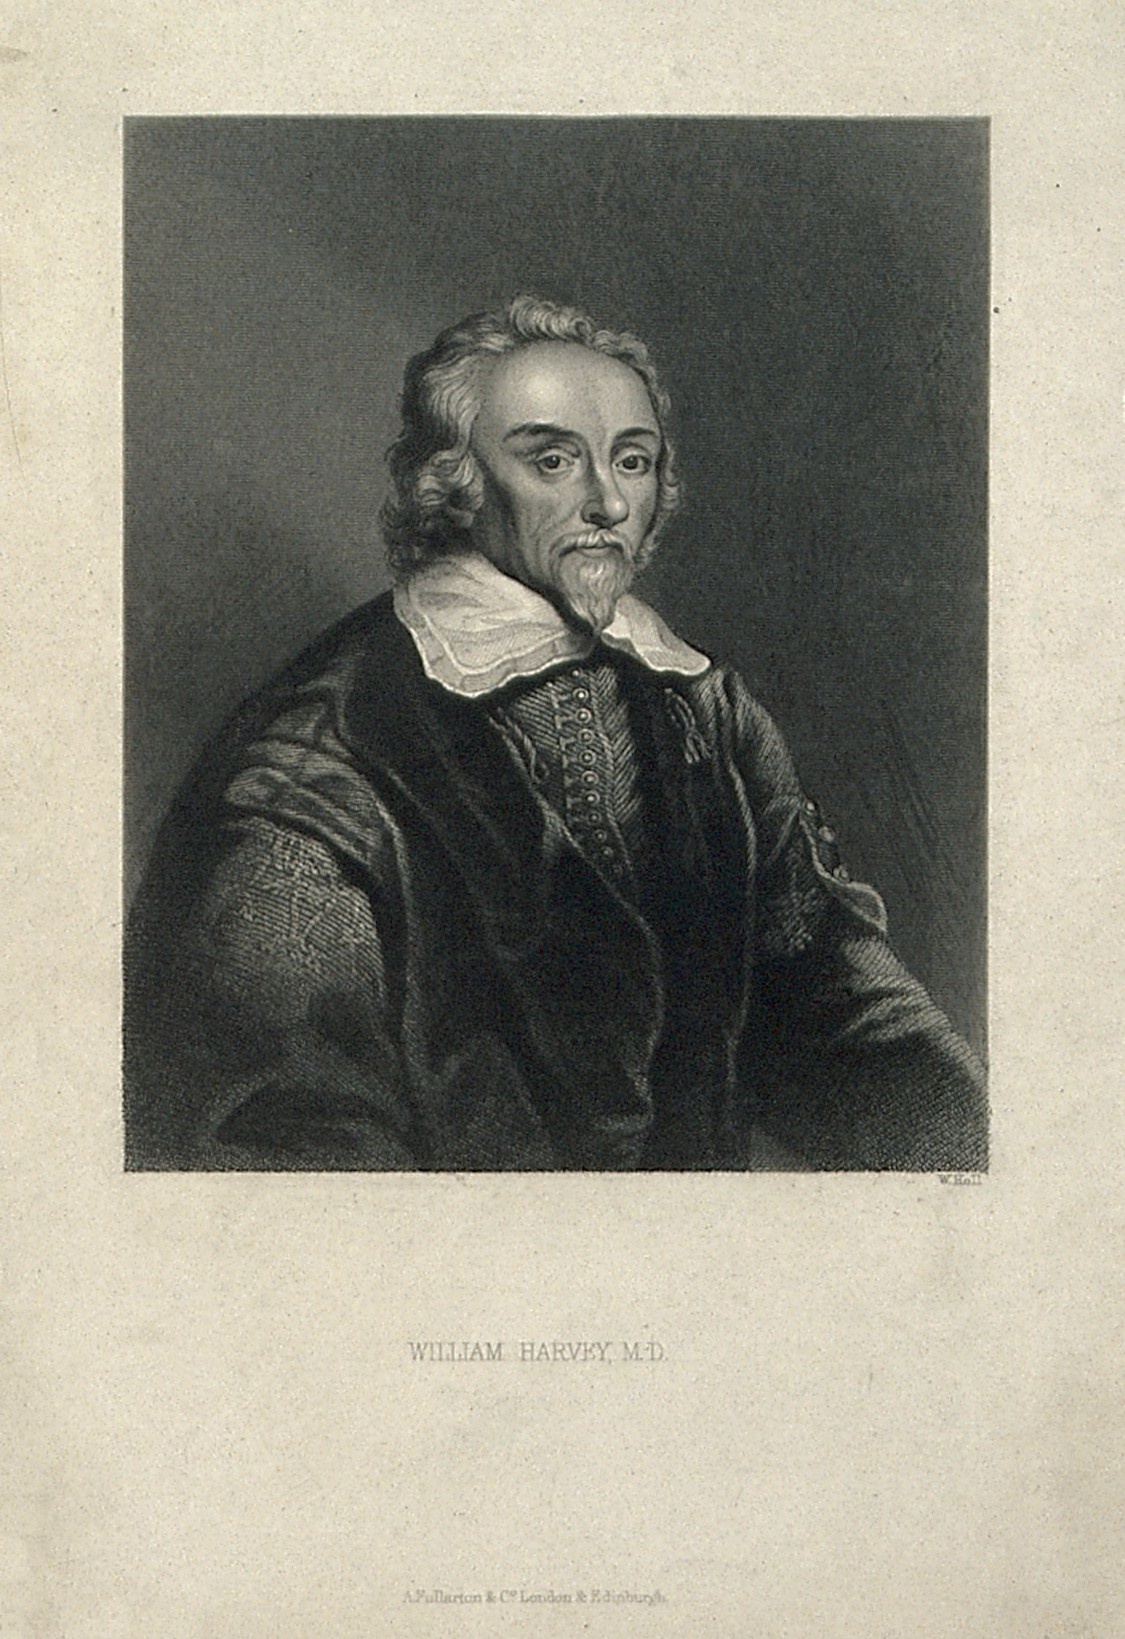
\includegraphics[width=0.3\linewidth]{images/book4/harvey.jpg}\hspace{0.05\linewidth}
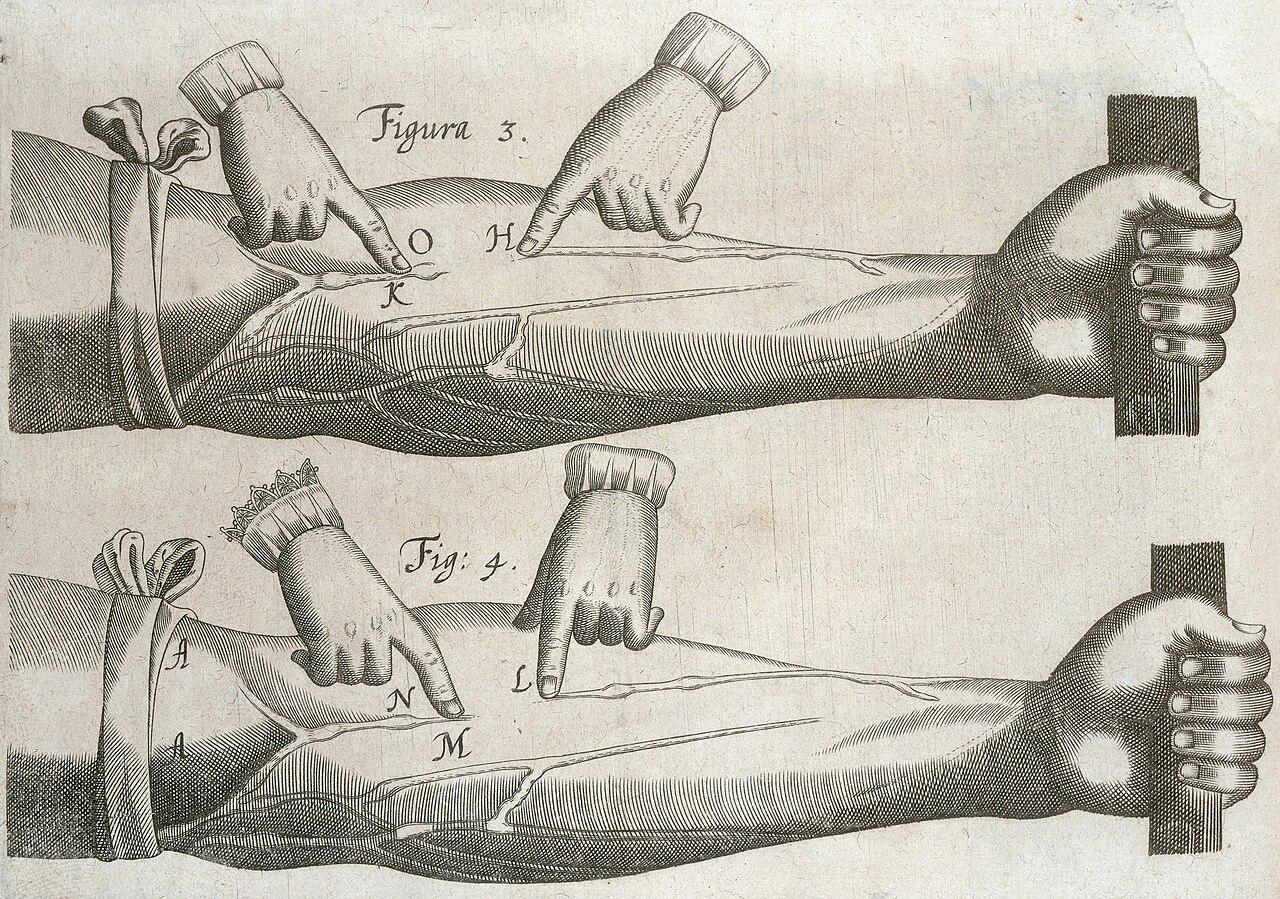
\includegraphics[width=0.42\linewidth]{images/book4/harvey-veins.jpg}

{\small 哈维，以及其 1628 年著作中的插图：
扎紧的前臂\omterm{def:b2:blood-circulation:vessels}{静脉}在绳扣下方肿胀，向手部压迫的\omterm{def:b2:blood-circulation:blood}{血液}
在瓣膜处被阻断。}
\end{omfigure}

\begin{omfigure}
\begin{tikzpicture}[every node/.style={font=\scriptsize}, >=stealth]
  % lungs and body
  \node[draw, rounded corners, fill=omDef!12, minimum width=3.4cm, minimum height=0.9cm] (lung) at (0,3) {肺：肺毛细血管};
  \node[draw, rounded corners, fill=omExo!25, minimum width=3.4cm, minimum height=0.9cm] (body) at (0,-3) {身体：体循环毛细血管};
  % heart chambers
  \node[draw, fill=omDef!25, minimum width=1.3cm, minimum height=0.7cm] (ra) at (-1.6,0.6) {右心房};
  \node[draw, fill=omDef!35, minimum width=1.3cm, minimum height=0.9cm] (rv) at (-1.6,-0.5) {右心室};
  \node[draw, fill=omThm!20, minimum width=1.3cm, minimum height=0.7cm] (la) at (1.6,0.6) {左心房};
  \node[draw, fill=omThm!35, minimum width=1.3cm, minimum height=0.9cm] (lv) at (1.6,-0.5) {左心室};
  \draw[->, thick] (ra) -- (rv); \draw[->, thick] (la) -- (lv);
  % pulmonary circuit
  \draw[->, very thick, omDef] (rv.west) -- ++(-1.4,0) |- (lung.west) node[pos=0.25, left, align=right] {肺动脉 \\\qty{25}{mmHg}};
  \draw[->, very thick, omThm] (lung.east) -| (la.east) node[pos=0.75, right, align=left] {肺静脉 \\含氧};
  % systemic circuit
  \draw[->, very thick, omThm] (lv.east) -- ++(1.4,0) |- (body.east) node[pos=0.25, right, align=left] {主动脉 \\\qty{120}{mmHg}};
  \draw[->, very thick, omDef] (body.west) -| (ra.west);
  \node[omDef, anchor=east, align=right] at (-2.45,-1.6) {腔静脉 \\\qty{5}{mmHg}};
  \node[anchor=north, align=center] at (0,-3.7) {两条循环中流量相同：\\\qty{5}{L/min}，静息时};
\end{tikzpicture}

{\small \omterm{def:b2:blood-circulation:circuits}{双循环}。右心将\omterm{def:b2:blood-circulation:blood}{血液}
以低压送经肺部；左心将\omterm{def:b2:blood-circulation:blood}{血液}
以高压送往全身；两个串联的泵
每分钟输送相同的血量。}
\end{omfigure}

\section{血管与流动的物理学}

\begin{definition}[血管树]\label{def:b2:blood-circulation:vessels}
\index{动脉}\index{小动脉}\index{毛细血管}\index{静脉}
\omterm{def:b2:blood-circulation:blood}{血液}经\emph{动脉}离开心脏：管壁厚的管道，
管壁含弹性层，每次搏动时扩张，搏动间隙回缩，
使脉搏变为较平稳的血流（主动脉
直径为\qty{2.5}{cm}）。它们分支为\emph{小动脉}，
是直径不超过十分之一毫米的血管，管壁主要为平滑肌：
通过收缩或舒张，小动脉改变其半径，
从而强烈地改变其阻力——小动脉是循环系统的“水龙头”，
也是大部分压降发生的部位。这些
血管通入\emph{毛细血管}：由单层内皮细胞
卷绕而成的管道，管腔直径为 \qtyrange{5}{10}{\micro m}，
长约 \qty{1}{mm}，全身约四百亿条，总表面积
接近 \qty{600}{m^2}，所有物质交换都在其管壁处进行。
毛细血管汇入微静脉和\emph{静脉}：管壁薄、
可扩张，在低压下容纳三分之二的\omterm{def:b2:blood-circulation:blood}{血液}，
瓣膜使血流朝向心脏，同时由肌肉挤压
它们。每条血管内壁都衬有一层
\emph{内皮}，它并非被动衬里，而是一个腺体——
它释放一氧化氮使小动脉舒张，并发出信号
招募白细胞，并且还是一道过滤器。
\end{definition}

\begin{omfigure}
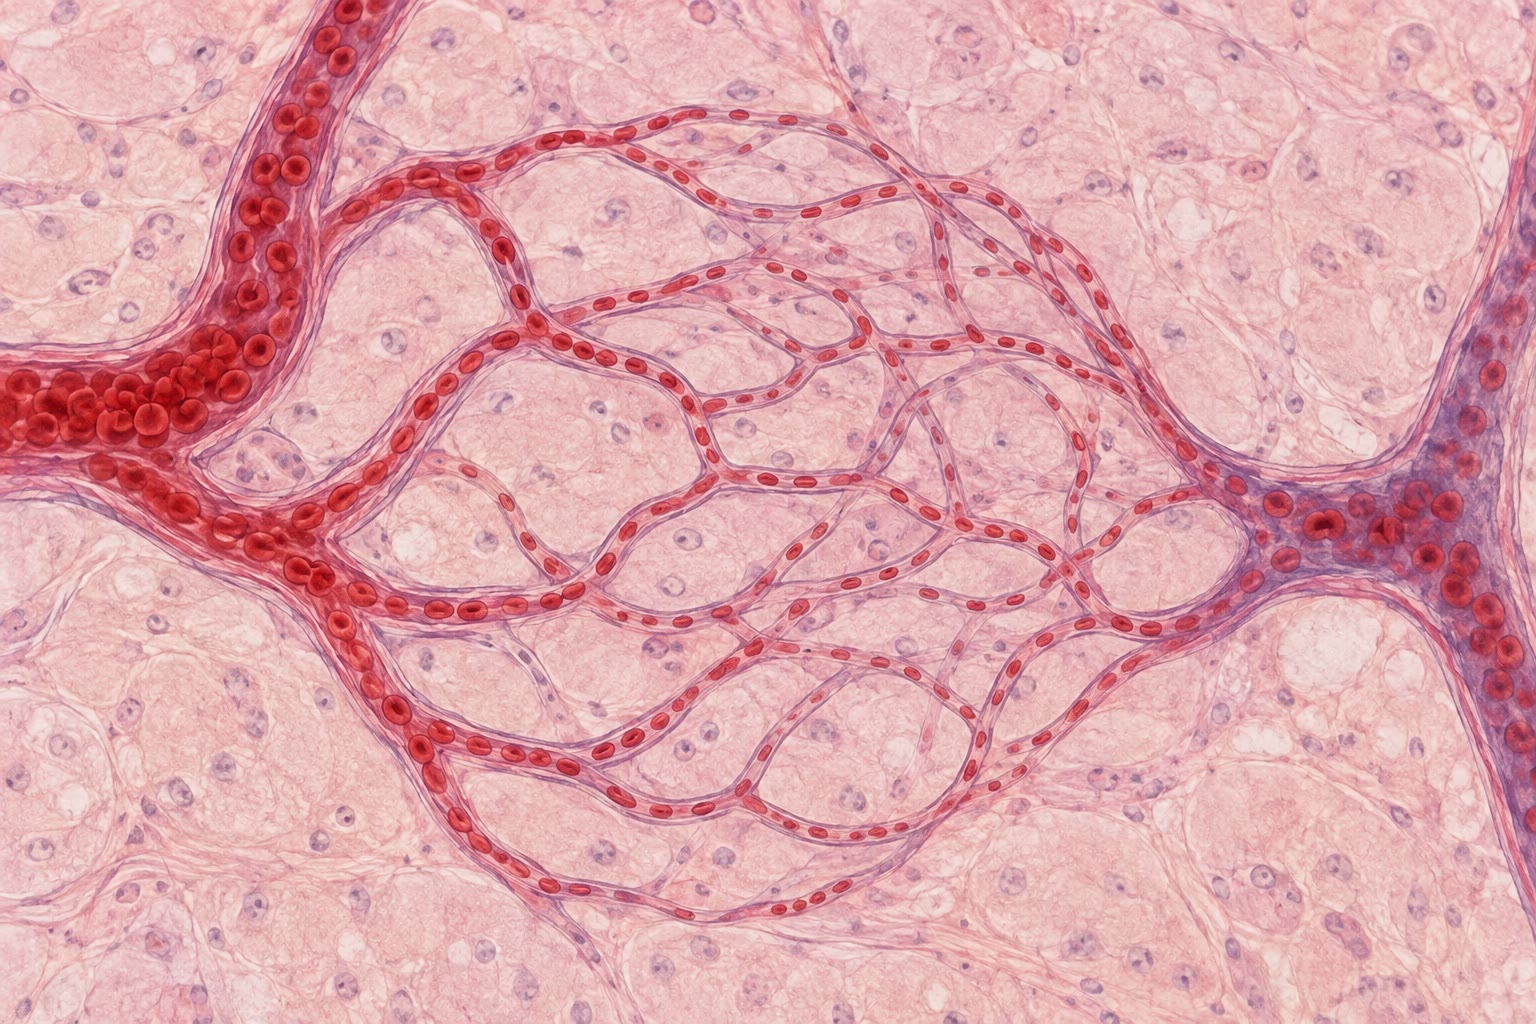
\includegraphics[width=0.55\linewidth]{images/book4/ai/b4-16-capillary-bed.jpg}

{\small \omterm{def:b2:blood-circulation:vessels}{毛细血管}床：\omterm{def:b2:blood-circulation:vessels}{小动脉}供血至\omterm{def:b2:blood-circulation:vessels}{毛细血管}网，
\omterm{def:b2:blood-circulation:blood}{红细胞}在其中单行通过，最终汇入微\omterm{def:b2:blood-circulation:vessels}{静脉}。}
\end{omfigure}

\begin{theorem}[泊肃叶定律与血管阻力]\label{thm:b2:blood-circulation:poiseuille}
\index{泊肃叶定律}\index{血管阻力}
流体流经管道的稳定流量 $Q$（流体黏度为 $\eta$）
管道半径为 $r$、长为 $L$，压差为 $\Delta P$，
由下式给出：
\[
Q = \frac{\pi r^{4}}{8\eta L}\,\Delta P, \qquad \text{ 从而 }\qquad
R \equiv \frac{\Delta P}{Q} = \frac{8\eta L}{\pi r^{4}} .
\]
阻力随半径的\emph{四次方}而减小：一条\omterm{def:b2:blood-circulation:vessels}{小动脉}若将半径缩小
\qty{20}{\%}，其阻力乘以
$1/0.8^{4} = 2.4$ 倍，若半径减半，则阻力增大 16 倍。这
正是为何\omterm{def:b2:blood-circulation:vessels}{小动脉}中几毫米的肌肉能够重新分配
全身的\omterm{def:b2:blood-circulation:blood}{血液}——进食后流向肠道，运动时流向
肌肉，高温时流向皮肤——也正是为何压强从
\omterm{def:b2:blood-circulation:vessels}{小动脉}处的 \qty{95}{mmHg} 降至\omterm{def:b2:blood-circulation:vessels}{毛细血管}入口处的 \qty{35}{mmHg}，
几乎全部降压发生在
\omterm{def:b2:blood-circulation:vessels}{小动脉}上，而沿主\omterm{def:b2:blood-circulation:vessels}{动脉}的降压
不足一毫米汞柱。
\end{theorem}
\begin{proof}
在稳定层流中，流体沿同心的圆柱壳层运动；其
壳层之间的黏性力与压力相平衡。
对半径为 $s < r$ 的圆柱体，压力为 $\pi s^{2}\Delta P$
等于其表面上的黏性阻力 $2\pi s L\,\eta\,(-\mathrm{d}v/
\mathrm{d}s)$，于是 $\mathrm{d}v/\mathrm{d}s = -s\Delta P/(2\eta L)$
并由 $v(r) = 0$，$v(s) = (\Delta P/4\eta L)(r^{2} - s^{2})$——一
条抛物线形的剖面。对截面上的速度积分，
$Q = \int_{0}^{r} v\,2\pi s\,\mathrm{d}s = (\pi\Delta P/2\eta L)
\int_{0}^{r}(r^{2}s - s^{3})\,\mathrm{d}s = \pi r^{4}\Delta P/8\eta
L$。（\omterm{def:b2:blood-circulation:blood}{血液}并非简单流体，\omterm{def:b2:blood-circulation:vessels}{动脉}也并非刚性，
但四次方定律已足以支撑整个机体的运转。）
\end{proof}

\begin{theorem}[连续性：血流在何处减慢]\label{thm:b2:blood-circulation:continuity}
\index{连续性方程}
每一级血管每秒通过的体积相同，因此
某一级的平均速度为 $v = Q/A$，其中 $A$ 为该级所有血管的\emph{总}
截面积。主\omterm{def:b2:blood-circulation:vessels}{动脉}
（\qty{3}{cm^2}）以 \qty{28}{cm/s} 的速度输送 \qty{5}{L/min} 的血流；
\omterm{def:b2:blood-circulation:vessels}{毛细血管}的总截面积接近 \qty{3000}{cm^2}，其流速
为 \qty{0.03}{cm/s}，因此一个\omterm{def:b2:blood-circulation:blood}{红细胞}需约三秒
穿过一根\omterm{def:b2:blood-circulation:vessels}{毛细血管}——这段时间足以使其氧气扩散出来
（见\cref{ch:b2:unicellular-diversity}：一微米
需一毫秒）。\omterm{def:b2:blood-circulation:vessels}{静脉}的总截面积小于
\omterm{def:b2:blood-circulation:vessels}{毛细血管}，使血流重新加速至 \qty{10}{cm/s}，在
腔\omterm{def:b2:blood-circulation:vessels}{静脉}中。血管树的构造使\omterm{def:b2:blood-circulation:blood}{血液}正好在
需要交换的地方减慢，而其余各处加快。
\end{theorem}
\begin{proof}
体积守恒：每秒进入某一级的量与离开的量相等，
因此 $Q = A\,v$ 在每一级都相同。$\qty{5}{L/min} =
\qty{83}{cm^3/s}$; $83/3 = \qty{28}{cm/s}$; $83/3000 =
\qty{0.028}{cm/s}$.
\end{proof}

\begin{omfigure}
\begin{tikzpicture}
\begin{axis}[
  width=0.9\linewidth, height=6.4cm,
  axis x line=bottom, axis y line=left,
  xmin=0, xmax=7, ymin=0, ymax=130,
  xtick={0.5,1.5,2.5,3.5,4.5,5.5,6.5},
  xticklabels={主动脉, 动脉, 小动脉, 毛细血管, 小静脉, 静脉, 腔静脉},
  x tick label style={font=\scriptsize, rotate=30, anchor=north east},
  ylabel={压强 (\unit{mmHg})}, ylabel style={font=\small, omThm},
  tick label style={font=\small}, ytick={0,40,80,120},
  legend style={font=\scriptsize, at={(0.97,0.95)}, anchor=north east, draw=none},
  clip=false,
]
\addplot[very thick, omThm] coordinates {(0,120) (0.5,118) (1,110) (1.5,100) (2,95) (2.5,60) (3,35) (3.5,25) (4,15) (4.5,12) (5,8) (5.5,5) (6,4) (6.5,3) (7,2)};
\addlegendentry{平均压强}
\addplot[very thick, omThm, dashed] coordinates {(0,120) (0.5,120) (1,125) (1.5,120) (2,100)};
\addplot[very thick, omThm, dashed] coordinates {(0,80) (0.5,80) (1,80) (1.5,82) (2,88)};
\addlegendentry{收缩压与舒张压}
\end{axis}
\begin{axis}[
  width=0.9\linewidth, height=6.4cm,
  axis x line=none, axis y line=right,
  xmin=0, xmax=7, ymin=0, ymax=32,
  ylabel={速度 (\unit{cm/s})}, ylabel style={font=\small, omDef},
  tick label style={font=\small}, ytick={0,10,20,30},
  legend style={font=\scriptsize, at={(0.97,0.72)}, anchor=north east, draw=none},
  clip=false,
]
\addplot[very thick, omDef] coordinates {(0,28) (0.5,26) (1,18) (1.5,10) (2,5) (2.5,1.5) (3,0.3) (3.5,0.03) (4,0.3) (4.5,1.5) (5,4) (5.5,7) (6,9) (6.5,10) (7,10)};
\addlegendentry{平均速度}
\end{axis}
\end{tikzpicture}

{\small 沿\omterm{def:b2:blood-circulation:circuits}{体循环}的压强（红色）与平均速度（蓝色）。
脉搏波在\omterm{def:b2:blood-circulation:vessels}{动脉}中被平滑，压强主要在
\omterm{def:b2:blood-circulation:vessels}{小动脉}处下降，\omterm{def:b2:blood-circulation:blood}{血液}在\omterm{def:b2:blood-circulation:vessels}{毛细血管}中流得最慢，
此处的总截面积是
主\omterm{def:b2:blood-circulation:vessels}{动脉}的一千倍。}
\end{omfigure}

\begin{theorem}[作为储库的弹性动脉]\label{thm:b2:blood-circulation:windkessel}
\index{Windkessel}\index{顺应性!动脉}\index{脉压}
心脏间歇性射血，组织获得的血流
近乎稳定。大\omterm{def:b2:blood-circulation:vessels}{动脉}起平滑作用：射血期间它们扩张，
储存一部分每搏输出量，舒张期则回缩，
推动\omterm{def:b2:blood-circulation:blood}{血液}前行。若\omterm{def:b2:blood-circulation:vessels}{动脉}具有\emph{顺应性}
$C$（单位压强下储存的体积），\omterm{def:b2:blood-circulation:vessels}{小动脉}具有
阻力 $R$，则在舒张期、主\omterm{def:b2:blood-circulation:vessels}{动脉}瓣关闭时，
压强按下式衰减：
\[
P(t) = P_{s}\,e^{-t/RC},
\]
因此持续 $t_d$ 的舒张期之后，舒张压为
$P_s e^{-t_d/RC}$。取 $R = \qty{1}{mmHg.s/mL}$，$C =
\qty{2}{mL/mmHg}$，$t_d = \qty{0.8}{s}$，则收缩压
\qty{120}{mmHg} 降至 \qty{80}{mmHg}。主\omterm{def:b2:blood-circulation:vessels}{动脉}较硬（$C$ 较小，
如老年时）使压强在两次搏动之间下降得更多，
射血期间升得更高：\emph{\omterm{thm:b2:blood-circulation:windkessel}{脉压}}增大，
心脏需克服更高的峰值压强做功。
\end{theorem}
\begin{proof}
舒张期内没有\omterm{def:b2:blood-circulation:blood}{血液}进入\omterm{def:b2:blood-circulation:vessels}{动脉}，\omterm{def:b2:blood-circulation:blood}{血液}经\omterm{def:b2:blood-circulation:vessels}{小动脉}流出，
流量为 $Q = P/R$；\omterm{def:b2:blood-circulation:vessels}{动脉}容积以
$\mathrm{d}V/\mathrm{d}t = -P/R$ 的速率减小，由于 $\mathrm{d}V = C\,
\mathrm{d}P$，有 $C\,\mathrm{d}P/\mathrm{d}t = -P/R$，其解为
时间常数为 $RC$ 的指数函数。取 $RC = \qty{2}{s}$，
则 $120\,e^{-0.4} = \qty{80}{mmHg}$。
\end{proof}

\section{毛细血管中的交换}

\begin{proposition}[两类交换]\label{prop:b2:blood-circulation:exchange}
\index{毛细血管交换}\index{斯塔林力}\index{水肿}\index{淋巴}
溶质穿过\omterm{def:b2:blood-circulation:vessels}{毛细血管}壁时，以\emph{扩散}方式移动——气体
和脂质穿过细胞，水和小分子溶质穿过
它们之间的缝隙，借助巨大的面积与很短的距离，
使通量足够大（菲克定律，与\omterm{def:b2:mammal-reproduction:placenta}{胎盘}的情形相同，见
\cref{ch:b2:mammal-reproduction}）——而水则以
\emph{整体流动}方式移动，由两种压强的平衡驱动。
\omterm{def:b2:blood-circulation:vessels}{毛细血管}内的静水压 $P_c$ 将液体推出；
\omterm{def:b2:blood-circulation:blood}{血浆}蛋白的\omterm{thm:b2:blood-circulation:oncotic}{胶体渗透压} $\pi_c$ 则将液体拉回
（\emph{\omterm{prop:b2:blood-circulation:exchange}{斯塔林力}}）。在\omterm{def:b2:blood-circulation:vessels}{动脉}端 $P_c \approx
\qty{35}{mmHg}$ 超过 $\pi_c \approx \qty{25}{mmHg}$，液体
向外滤过；在\omterm{def:b2:blood-circulation:vessels}{静脉}端 $P_c \approx \qty{15}{mmHg}$，液体
被重吸收。全身每天约有 \qty{20}{L} 滤出，
\qty{17}{L} 回流，余下的 \qty{3}{L} 连同漏出的
蛋白质由\emph{\omterm{prop:b2:blood-circulation:exchange}{淋巴}管}收集，
并在颈部回注入\omterm{def:b2:blood-circulation:vessels}{静脉}。\emph{\omterm{prop:b2:blood-circulation:exchange}{水肿}}——组织液
积聚所致的肿胀——每当平衡打破时便会出现：
\omterm{def:b2:blood-circulation:vessels}{静脉}压过高（心力衰竭）、\omterm{def:b2:blood-circulation:blood}{血浆}蛋白过低
（饥饿、肝或肾脏疾病）、\omterm{def:b2:blood-circulation:vessels}{毛细血管}渗漏
（炎症）或\omterm{prop:b2:blood-circulation:exchange}{淋巴}回流受阻。
\end{proposition}

\begin{omfigure}
\begin{tikzpicture}[every node/.style={font=\scriptsize}, >=stealth]
  % capillary
  \draw[thick, fill=omThm!10] (0,0) rectangle (9,1.2);
  \node[left] at (-0.1,0.6) {小动脉};
  \node[right] at (9.1,0.6) {小静脉};
  \draw[->, very thick, omThm] (0.3,0.6) -- (8.7,0.6);
  % pressures
  \node[above, align=center] at (1.5,1.3) {动脉端 \\$P_c = 35$，$\pi_c = 25$};
  \node[above, align=center] at (7.5,1.3) {静脉端 \\$P_c = 15$，$\pi_c = 25$};
  \foreach \x in {0.8,1.5,2.2} \draw[->, thick, omDef] (\x,0) -- (\x,-0.7);
  \node[below, align=center, omDef] at (1.5,-0.75) {净 $+10$ mmHg：\\滤过};
  \foreach \x in {6.8,7.5,8.2} \draw[->, thick, omDef] (\x,-0.7) -- (\x,0);
  \node[below, align=center, omDef] at (7.5,-0.75) {净 $-10$ mmHg：\\重吸收};
  \draw[->, thick, omExo!70!black] (4.5,-0.4) -- (4.5,-1.6) node[below, align=center] {进入淋巴的多余液体：\\\qty{3}{L} 每天};
  \node[align=center] at (4.5,-0.15) {组织液};
\end{tikzpicture}

{\small 沿\omterm{def:b2:blood-circulation:vessels}{毛细血管}的 Starling 力。静水压
把液体推出去，\omterm{def:b2:blood-circulation:blood}{血浆}蛋白的\omterm{thm:b2:blood-circulation:oncotic}{胶体渗透压}把它拉回；
\omterm{def:b2:blood-circulation:vessels}{动脉}端的滤过量超过\omterm{def:b2:blood-circulation:vessels}{静脉}端的重吸收量，
多余部分由\omterm{prop:b2:blood-circulation:exchange}{淋巴}带回。}
\end{omfigure}

\begin{theorem}[胶体渗透压]\label{thm:b2:blood-circulation:oncotic}
\index{胶体渗透压}\index{白蛋白}
设 $c$ 摩尔每升的某种溶质不能穿过膜，
则它在膜两侧产生的渗透压为 $\pi = cRT$（
范托夫）。\omterm{def:b2:blood-circulation:blood}{血浆}\omterm{thm:b2:blood-circulation:oncotic}{白蛋白}浓度为 \qty{40}{g/L}，是摩尔质量为
\qty{66}{kg/mol} 的蛋白质，故 $c = \qty{0.6}{mmol/L}$，$\pi =
0.6\times 8.314\times 310 = \qty{1.55}{kPa} \approx \qty{12}{mmHg}$;
其他蛋白质，以及\omterm{thm:b2:blood-circulation:oncotic}{白蛋白}负电荷所保留的额外离子，
使总量约为 \qty{25}{mmHg}。\omterm{def:b2:blood-circulation:blood}{血浆}中的氯化钠，
浓度为 \qty{150}{mmol/L}，若按同样方法计算，它将产生
\qty{5800}{mmHg}——但它能自由穿过\omterm{def:b2:blood-circulation:vessels}{毛细血管}壁，
因而在壁两侧不产生渗透压。对\omterm{def:b2:blood-circulation:vessels}{毛细血管}起作用的是蛋白质：
\omterm{thm:b2:blood-circulation:oncotic}{白蛋白}减半时，例如肾病患者经尿液丢失\omterm{thm:b2:blood-circulation:oncotic}{白蛋白}，
重吸收的拉力随之减半，液体在组织中积聚，
患者便出现\omterm{prop:b2:blood-circulation:exchange}{水肿}。
\end{theorem}
\begin{proof}
$\qty{40}{g/L}/\qty{66000}{g/mol} = \qty{6.1e-4}{mol/L} =
\qty{0.61}{mol/m^3}$; $\pi = cRT = 0.61\times 8.314\times 310 =
\qty{1570}{Pa}$；$\qty{1}{mmHg} = \qty{133}{Pa}$，故为 \qty{11.8}{mmHg}。
范托夫定律本身，是在本科一年级分册中导出的
稀溶液极限情形。
\end{proof}

\begin{example}[作为运输系统的循环]\label{ex:b2:blood-circulation:transport}
每分钟五升\omterm{def:b2:blood-circulation:blood}{血液}流经 \qty{600}{m^2} 的\omterm{def:b2:blood-circulation:vessels}{毛细血管}壁，是无与伦比的
输送系统。它在几个细胞直径之内把氧气送到每个细胞
（身体中没有哪个细胞距\omterm{def:b2:blood-circulation:vessels}{毛细血管}超过
\qty{20}{\micro m}），带走其 $\mathrm{CO_2}$，
乳酸和尿素，把肝脏的葡萄糖运到脑，
把脂肪储备中的脂肪酸运到肌肉，
把\cref{ch:b2:cell-signalling}中的激素从一个腺体在一分钟内送到全身每个
受体，并把身体核心的热量输送到
皮肤再送回，并在
数小时内把白细胞运到伤口。它也是脆弱之处：一个血栓、一次出血或一个
衰竭的泵会使这一切同时中止，而脑几乎不储存燃料，
几秒钟内便会失效。本部分的其余内容
讨论泵（\cref{ch:b2:heart}），以及血压如何调节，
以保证这一输送在站立、奔跑和失血时仍能持续
（\cref{ch:b2:blood-pressure}）。
\end{example}

\section{练习}

\begin{exercise}[$\star$]\label{exo:b2:blood-circulation:1}
给出\omterm{def:b2:blood-circulation:blood}{血液}按体积计的组成，以及每种细胞成分的数量、大小和
功能。
\end{exercise}

\begin{exercise}[$\star$]\label{exo:b2:blood-circulation:2}
画出鱼类和哺乳动物的循环回路，标出各处压强，并
说明\omterm{def:b2:blood-circulation:circuits}{双循环}获得了什么。
\end{exercise}

\begin{exercise}[$\star$]\label{exo:b2:blood-circulation:3}
对每种血管类型——\omterm{def:b2:blood-circulation:vessels}{动脉}、\omterm{def:b2:blood-circulation:vessels}{小动脉}、\omterm{def:b2:blood-circulation:vessels}{毛细血管}、\omterm{def:b2:blood-circulation:vessels}{静脉}——给出
血管壁的结构及其所起的作用。
\end{exercise}

\begin{exercise}[$\star$]\label{exo:b2:blood-circulation:4}
从数量出发，用现代数值重建哈维的论证：
每搏 \qty{70}{mL}，每分钟 \num{72} 次搏动，\omterm{def:b2:blood-circulation:blood}{血液} \qty{5}{L}。
\end{exercise}

\begin{exercise}[$\star\star$]\label{exo:b2:blood-circulation:5}
计算主\omterm{def:b2:blood-circulation:vessels}{动脉}（半径 \qty{1.25}{cm}，
长 \qty{40}{cm}，$\eta = \qty{3e-3}{Pa.s}$），流量为
\qty{5}{L/min} 时沿程的压降，依泊肃叶定律计算，分别以帕斯卡和毫米汞柱表示，并加以评论。
\end{exercise}

\begin{exercise}[$\star\star$]\label{exo:b2:blood-circulation:6}
半径为 \qty{15}{\micro m} 的\omterm{def:b2:blood-circulation:vessels}{小动脉}收缩至
\qty{12}{\micro m}，随后扩张至 \qty{20}{\micro m}。两种情形下，其阻力各变为原来的
多少倍，并求在
压强不变时其流量如何变化？
\end{exercise}

\begin{exercise}[$\star\star$]\label{exo:b2:blood-circulation:7}
主\omterm{def:b2:blood-circulation:vessels}{动脉}的截面积为 \qty{3}{cm^2}，\omterm{def:b2:blood-circulation:vessels}{毛细血管}的
总截面积为 \qty{3000}{cm^2}，流量为 \qty{5}{L/min}。计算
两者中的平均流速，以及一个\omterm{def:b2:blood-circulation:blood}{红细胞}在
\qty{1}{mm} 长的\omterm{def:b2:blood-circulation:vessels}{毛细血管}中所用的时间。运动时心输出量升至
\qty{25}{L/min}，且肌肉\omterm{def:b2:blood-circulation:vessels}{毛细血管}开放，
通过时间会发生什么变化？
\end{exercise}

\begin{exercise}[$\star\star$]\label{exo:b2:blood-circulation:8}
已知两端的 $P_c = 35$ 和 \qty{15}{mmHg}，$\pi_c =
\qty{25}{mmHg}$，组织压强可忽略，计算
两端的净滤过压。若\omterm{def:b2:blood-circulation:vessels}{静脉}压升高，
使\omterm{def:b2:blood-circulation:vessels}{静脉}端的 $P_c$ 为 \qty{28}{mmHg}，会发生什么？
\end{exercise}

\begin{exercise}[$\star\star$]\label{exo:b2:blood-circulation:9}
计算 \qty{40}{g/L} \omterm{thm:b2:blood-circulation:oncotic}{白蛋白}（
\qty{66}{kg/mol}）在 \qty{37}{\celsius} 时的\omterm{thm:b2:blood-circulation:oncotic}{胶体渗透压}，以及 \qty{20}{g/L} \omterm{thm:b2:blood-circulation:oncotic}{白蛋白}的\omterm{thm:b2:blood-circulation:oncotic}{胶体渗透压}。为什么
\omterm{def:b2:blood-circulation:blood}{血浆}中浓度为 \qty{150}{mmol/L} 的钠，对
Starling 平衡没有任何贡献？
\end{exercise}

\begin{exercise}[$\star\star\star$]\label{exo:b2:blood-circulation:10}
已知 $R = \qty{1}{mmHg.s/mL}$，$C = \qty{2}{mL/mmHg}$，计算
从收缩压 \qty{120}{mmHg} 出发、经过 \qty{0.8}{s} 后的
舒张压。对顺应性减半的主\omterm{def:b2:blood-circulation:vessels}{动脉}重新计算。解释为何
老年人的\omterm{thm:b2:blood-circulation:windkessel}{脉压}较宽，以及这对
心脏造成了什么代价。
\end{exercise}

\begin{exercise}[$\star\star\star$]\label{exo:b2:blood-circulation:11}
\omterm{def:b2:blood-circulation:circuits}{体循环}阻力为 $R = (P_{\text{动脉}} - P_{\text{静脉}})/Q$。
分别计算静止时（$95 - 5$ mmHg，\qty{5}{L/min}）与运动时
（$110 - 5$，\qty{25}{L/min}）的阻力。若\omterm{def:b2:blood-circulation:vessels}{小动脉}承担全部阻力，平均\omterm{def:b2:blood-circulation:vessels}{小动脉}半径
需改变为原来的多少倍？
\end{exercise}

\begin{exercise}[$\star\star\star$]\label{exo:b2:blood-circulation:12}
“循环系统的构造使\omterm{def:b2:blood-circulation:blood}{血液}在必须进行物质交换的地方流动缓慢，
而在其他各处流动迅速。”请结合\omterm{thm:b2:blood-circulation:continuity}{连续性方程}、
泊肃叶定律与血管树的几何结构加以讨论，并说明
为何\omterm{def:b2:blood-circulation:circuits}{开放式循环}无法做到同样的事。
\end{exercise}

\section{问题：数字中的循环系统}

\begin{problem}[{周末问题——哈维总量的重算，
用泊肃叶定律与连续性方程计算血管树的压强与速度，
平衡毛细血管每日的滤过量，
对主动脉的缓冲作用建模，
并以心输出量、小动脉压降、当日滤液量与舒张压作结。}]
\label{pb:b2:blood-circulation:1}
数据：每搏输出量 \qty{70}{mL}，心率 \qty{72}{min^{-1}}，
血容量 \qty{5}{L}，$\eta = \qty{3e-3}{Pa.s}$，$\qty{1}{mmHg} =
\qty{133}{Pa}$。主\omterm{def:b2:blood-circulation:vessels}{动脉}：半径 \qty{1.25}{cm}，长度 \qty{40}{cm}。
\omterm{def:b2:blood-circulation:vessels}{小动脉}：$3\times 10^{6}$ 条并联，每条半径
\qty{15}{\micro m}，长度 \qty{1}{mm}。\omterm{def:b2:blood-circulation:vessels}{毛细血管}：$4\times
10^{10}$，半径 \qty{3}{\micro m}，长度 \qty{1}{mm}，其中四分之一
静止时开放。斯塔林平衡：$P_c$ 沿一条
\omterm{def:b2:blood-circulation:vessels}{毛细血管}由 35 降至 \qty{15}{mmHg}，$\pi_c = \qty{25}{mmHg}$。风箱模型：$C =
\qty{2}{mL/mmHg}$，舒张期 \qty{0.8}{s}。

\medskip
\noindent\textbf{第一部分——哈维的总量。}
\begin{enumerate}
  \item 分别以升每分钟和升每天为单位，计算心输出量。
  \item 全部血容量一天内循环多少次？
  \item 哈维估计每搏输出 2~盎司（\qty{57}{g}），
        其中他假定至少四分之一被射出，心率为每分钟 72
        次。由此算得的每小时\omterm{def:b2:blood-circulation:blood}{血液}质量是多少，
        它与一个人的体重相比又如何？
  \item 这一论证为何支持循环，而非
        持续生产与消耗的观点？
  \item 描述结扎实验，以及瓣膜所显示的结果。
  \item 哈维未能看到的是什么？又是谁看到了它？
\end{enumerate}

\medskip
\noindent\textbf{第二部分——血管树。}
\begin{enumerate}[resume]
  \item 计算主\omterm{def:b2:blood-circulation:vessels}{动脉}中的平均速度。
  \item 用泊肃叶定律计算主\omterm{def:b2:blood-circulation:vessels}{动脉}上的压降，
        以 mmHg 为单位。
  \item 计算一条\omterm{def:b2:blood-circulation:vessels}{小动脉}的阻力，以及 $3\times
        10^{6}$ 条并联时的阻力。
  \item 计算静止时输出量下\omterm{def:b2:blood-circulation:vessels}{小动脉}上的压降，
        以 mmHg 为单位。
  \item 计算开放\omterm{def:b2:blood-circulation:vessels}{毛细血管}的总截面，以及其中
        的平均速度；再求\omterm{def:b2:blood-circulation:blood}{血液}流过一根\omterm{def:b2:blood-circulation:vessels}{毛细血管}的通过时间。
  \item \omterm{def:b2:blood-circulation:vessels}{小动脉}收缩，使其半径下降
        \qty{10}{\%}。重新计算压降。心脏须如何
        做，才能维持相同的心输出量？
\end{enumerate}

\medskip
\noindent\textbf{第三部分——\omterm{def:b2:blood-circulation:vessels}{毛细血管}。}
\begin{enumerate}[resume]
  \item 计算\omterm{def:b2:blood-circulation:vessels}{动脉}端的净滤过压、
        \omterm{def:b2:blood-circulation:vessels}{静脉}端与中点处的净滤过压（设 $P_c$
        沿程线性下降）。
  \item 将\omterm{def:b2:blood-circulation:vessels}{毛细血管}分为滤过半段与重吸收半段，
        估算全身每日被滤过与被重吸收的液体量，
        取各半段上平均净压为
        $+10$ 与
        \qty{-8.5}{mmHg}，两半段各以每日每 mmHg
        \qty{2}{L} 的速率转移液体。
  \item 由此推算\omterm{prop:b2:blood-circulation:exchange}{淋巴}流量。
  \item \omterm{def:b2:blood-circulation:blood}{血浆}\omterm{thm:b2:blood-circulation:oncotic}{白蛋白}降至 \qty{20}{g/L}。重新计算 $\pi_c$
        （假设其随\omterm{thm:b2:blood-circulation:oncotic}{白蛋白}成比例变化），以及
        两端的净压。会发生什么？
  \item \omterm{def:b2:blood-circulation:vessels}{静脉}压升高，使 $P_c$ 由 35
        变至 \qty{28}{mmHg}。重新计算平均净压与
        每日平衡。液体去向何处？
  \item 计算\omterm{def:b2:blood-circulation:vessels}{毛细血管}的总表面积（按圆柱体计，
        全部计入），以及一个分子扩散到
        距\omterm{def:b2:blood-circulation:vessels}{毛细血管} \qty{20}{\micro m} 处的细胞所需的时间（$D = \qty{1e-9}{m^2/s}$）。
\end{enumerate}

\medskip
\noindent\textbf{第四部分——作为储库的主\omterm{def:b2:blood-circulation:vessels}{动脉}。}
\begin{enumerate}[resume]
  \item 根据平均压为
        \qty{93}{mmHg}、\omterm{def:b2:blood-circulation:vessels}{静脉}压 \qty{3}{mmHg} 及静止时输出量，
        计算\omterm{def:b2:blood-circulation:circuits}{体循环}阻力，以 \unit{mmHg.s/mL} 为单位。
  \item 计算时间常数 $RC$，以及
        以收缩压 \qty{120}{mmHg} 出发，经过 \qty{0.8}{s} 后的舒张压。
  \item 对 $C = \qty{1}{mL/mmHg}$ 重新计算，
        \omterm{thm:b2:blood-circulation:windkessel}{脉压}发生了什么变化？
  \item 心率升至 \num{120}，舒张期缩短至
        \qty{0.3}{s}，计算舒张压。
  \item 射出的 \qty{70}{mL} 中，有多少在收缩期储存于
        \omterm{def:b2:blood-circulation:vessels}{动脉}中（若压强升高
        \qty{20}{mmHg}）？其余去向何处？
  \item 说明为何在舒张期充盈的冠状\omterm{def:b2:blood-circulation:vessels}{动脉}
        依赖主\omterm{def:b2:blood-circulation:vessels}{动脉}的弹性回缩。
  \item 给出结果：心输出量、\omterm{def:b2:blood-circulation:vessels}{小动脉}
        压降、当日净滤液量与舒张压，
        分别对应 $C = 2$ 与 $C = 1$。
\end{enumerate}
\end{problem}
